\section{Exercises}

%__________________
\subsection{Variability in estimates}

% 1

\eoce{\qt{Identify the parameter, Part I} For each of the following situations, state whether the parameter of interest is a mean or a proportion. All questions were asked in the BRFSS questionnaire in 2000. It may be helpful to examine whether individual responses are numerical or categorical.
\begin{parts}
\item The BRFSS respondents were asked, "For how many days during the past 30 days was your physical health not good." 
\item The BRFSS respondents were asked, "During the past 12 months, was there any time that you did not have any health insurance or coverage?"
\item The BRFSS respondents were asked, "During the past month, did you participate in any physical activities or exercises such as running, calisthenics, golf, gardening, or walking for exercise?"
\item As a followup question, they were asked "How far did you usually walk/run/jog/swim?"
\item The BRFSS respondents were asked, "On the average, when you smoked during the past 30 days, about how many cigarettes did you smoke a day?"
\end{parts}
}{}

% 2

\eoce{\qt{Identify the parameter, Part II} For each of the following situations, state whether the parameter of interest is a mean or a proportion. Again, the following questions were asked in the BRFSS questionnaire in 2000. 
\begin{parts}
\item The BRFSS respondents were asked, "Are you now trying to lose weight?"
\item The BRFSS respondents were asked, "About how much do you weigh without your shoes?"
\item The BRFSS respondents were asked, "How much would you like to weigh?"
\item The BRFSS respondents were asked, "Have you ever served on active duty in the United States Armed Forces, either in the regular military or in a National Guard or military reserve unit?"
\item The BRFSS respondents were asked, "How many children live in your household who are less than 5 years old?"
\item The female BRFSS respondents were asked, "A Pap smear is a test for cancer of the cervix. Have you ever had a Pap smear?"
\item The BRFSS respondents were asked, "How many residential telephone numbers do you have?"
\end{parts}
}{}

% 3

\eoce{\qt{Frog Study} \label{frog} Recall the Frog Study introduced in Chapter~\ref{introductionToData} and published in the \textit{Journal of Evolutionary Biology}.\footnote{ Chen, W., et al. Maternal investment increases with altitude in a frog on the Tibetan Plateau. Journal of evolutionary biology 26.12 (2013): 2710-2715.} Below is a histogram of the distribution of body size of mother female frogs (\textit{Rana kukunoris}). Sample statistics for this distribution are also provided.\\
\begin{minipage}[c]{0.7\textwidth}
\begin{center}
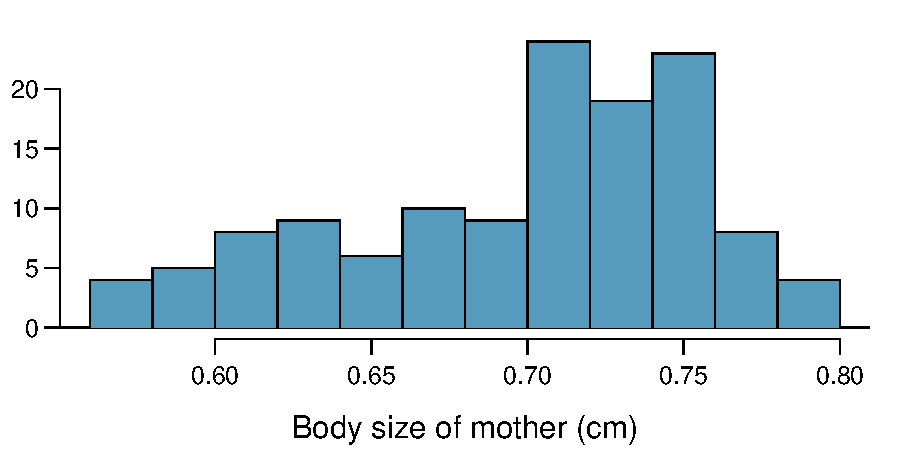
\includegraphics[width=96mm]{ch_inference_foundations_oi_biostat/figures/eoce/frogs/frogs}
\end{center}
\end{minipage}
\begin{minipage}[c]{0.3\textwidth}
\begin{center}
% latex table generated in R 3.1.1 by xtable 1.7-4 package
% Sat Nov  7 14:53:33 2015
\begin{tabular}{l|rr l}
Min. & 0.56 \\ 
  1st Qu. & 0.67 \\ 
  Median & 0.72 \\ 
  Mean & 0.70 \\ 
  3rd Qu. & 0.75 \\ 
  Max. & 0.79 \\ 
  SD. & 0.06\\
\end{tabular}
\end{center}
\end{minipage}
\begin{parts}
\item What is the point estimate for the average body size of the \textit{Rana kukunoris} mother? What is the point estimate for the median?
\item What is the point estimate for the standard deviation? How about the IQR?
\item Imagine if scientists observed a mother with a body size of 0.86 cm. Is this unusual? How about a mother with a body size of 0.6? \textit{Hint:} Consider observations farther than two standard deviations from the mean to be unusual.
\item Other scientists decide to replicate the study and take a random sample of 129 \textit{Rana kukunoris} frogs, the same number of frogs as in the original study. They measure the female body sizes and calculate a sample mean of 0.72 cm. The scientists decide that the original study is invalidated because the sample means differ. Is this correct? Explain. 
\item Scientists in part (d) observed variation among samples. What is a measure introduced in Chapter~\ref{foundationsForInference} for this variability in point estimates? Calculate this value from the original study. \end{parts}
}{}

% 4

\eoce{\qt{Heights of adults, Part I}\label{adultheights} \label{heights} Researchers studying anthropometry collected body girth measurements and skeletal diameter measurements, as well as age, weight, height and gender, for 507 physically active individuals. The histogram below shows the sample distribution of heights in centimeters. \footfullcite{Heinz:2003} \\
\begin{minipage}[c]{0.7\textwidth}
\begin{center}
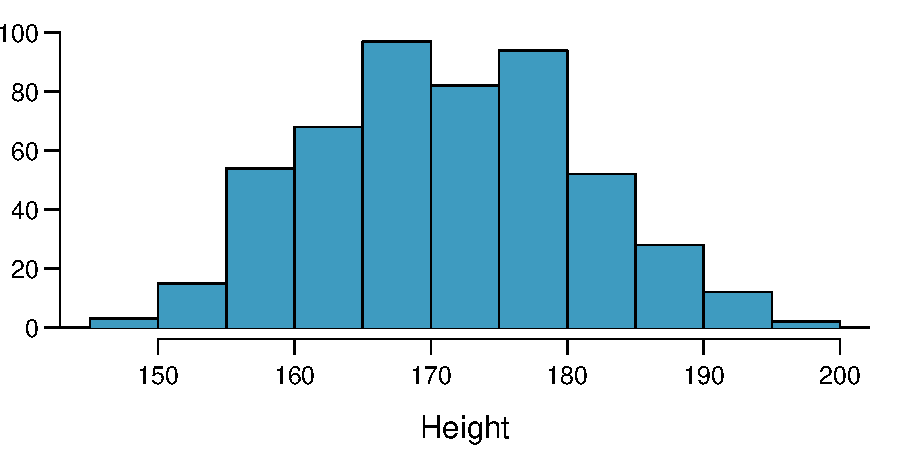
\includegraphics[width=85mm]{ch_inference_foundations_oi_biostat/figures/eoce/bdims/bdims_heights}
\end{center}
\end{minipage}
\begin{minipage}[c]{0.3\textwidth}
\begin{center}
\begin{tabular}{l|r l}
Min		& 147.2 \\
Q1		& 163.8 \\
Median	& 170.3 \\
Mean	& 171.1 \\
SD		&  9.4 \\
Q3		& 177.8 \\
Max		& 198.1 \\
\end{tabular}
\end{center}
\end{minipage}
\begin{parts}
\item What is the point estimate for the average height of active individuals? What about the median?
\item What is the point estimate for the standard deviation of the heights of active individuals? What about the IQR?
\item Is a person who is 1m 80cm (180 cm) tall considered unusually tall? And is a person who is 1m 55cm (155cm) considered unusually short? Explain your reasoning.
\item The researchers take another random sample of physically active individuals. Would you expect the mean and the standard deviation of this new sample to be the ones given above? Explain your reasoning.
\item The sample means obtained are point estimates for the mean height of all active individuals, if the sample of individuals is equivalent to a simple random sample. What measure do we use to quantify the variability of such an estimate? Compute this quantity using the data from the original sample under the condition that the data are a simple random sample. 
\end{parts}
}{}

% 5
\eoce{\qt{FAMuSS Part I}\label{famusspt1} The Functional polymorphisms Associated with Human Muscle Size and Strength study (FAMuSS), funded by the National Institutes of Health (NIH), studied the \textit{actn3} gene that produces a protein to regular fast muscle fibers and its association with size and strength of muscle before and after exercise. They measured a variety of characteristics including age and BMI of college students.\footnote{Thompson PD, Moyna M, Seip, R, et al., 2004.  Functional Polymorphisms Associated with Human Muscle Size and Strength.  Medicine and Science in Sports and Exercise 36:1132 - 1139} 
\begin{center}
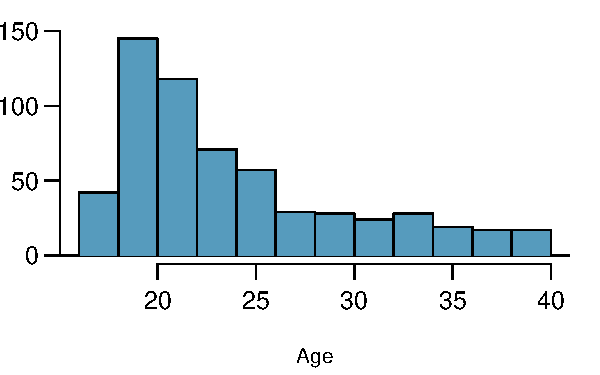
\includegraphics[width=0.7\textwidth]{ch_inference_foundations_oi_biostat/figures/eoce/famussage/famussage}
\end{center}
\begin{parts}
\item The mean age of the participants is 24.40 and the standard deviation of the sample is 5.81 years. What is missing to calculate the standard error?
\item The sample contains 595 participants. How much variability should the researchers expect in the mean age of repeated samples? 
\item The distribution of ages is skewed to the right. Is the sampling distribution of the sample mean nearly normal?
\item The Census claims that the average age of college students is 24.34.\footnote{\url{https://www.census.gov/hhes/school/data/cps/historical/TableA-6.xls}} Is an average of 24.34 consistent with the FAMuSS sample?
\end{parts}
}{}

%6
\eoce{\qt{Gifted children, Part I} \label{giftedpt1} Researchers investigating characteristics of gifted children collected data from schools in a large city on a random sample of thirty-six children who were identified as gifted children soon after they reached the age of four. The following histograms shows the distribution of IQs from mother and father. \footfullcite{Graybill:1994}

\begin{center}
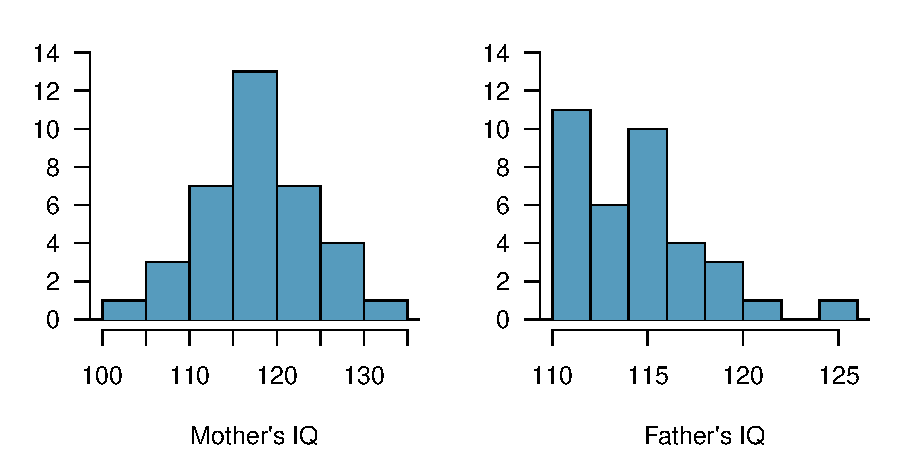
\includegraphics[width=\textwidth]{ch_inference_foundations_oi_biostat/figures/eoce/gifted/parentIQ} 
\end{center}

\begin{parts}
\item The researchers want to estimate the average difference between mother and father IQ. What would be a reasonable point estimate for this?
\item The sample mean of the mother IQ is 118.17, and the sample mean for the father IQ is 114.78. What is the point estimate of the difference in mother and father IQ. 
\item The standard deviation for mother IQ is 6.50, and the standard deviation for father IQ is 3.48. What is the standard error for the difference between mother and father IQ? 
\item Are there any key features about this study that the researchers need to be aware of when calculating the average difference in parent IQ? 
\end{parts}
}{}

% 7

\eoce{\qt{Heights of adults, Part II} The researchers from Exercise~\ref{adultheights} want to present their findings. The conference that they are presenting to is in the U.S., and much of the research is in Imperial. 
\begin{parts}
\item Do the researchers need to remeasure the 507 individuals again in inches? Why or why not?
\item What is the sample mean of the heights? What about the median? 
\item If the researchers observed 100 individuals instead of 507, is the standard error expected to be larger or smaller? 
\end{parts}
}{}

% 8
\eoce{\qt{FAMuSS Part II}\label{famusspt2} Recall the FAMuSS study introduced in Exercise~\ref{famusspt1}. Researchers, Team B, decide to sample 5,000 college students instead of the 595 that the researchers, Team A, in Exercise~\ref{famusspt1} did. 
\begin{parts}
\item Which team will tend to observe the larger standard deviation? Is it unknown?
\item Which team will observe a larger standard error? Is it unknown? 
\item Which team is likely to get the older sample, on average? Is it unknown? 
\item Which team is likely to get the younger sample, on average? Is it unknown? 
\end{parts}
}{}


%__________________
\subsection{Confidence intervals}

% 9

\eoce{\qt{Relaxing after work} \label{relax} The General Social Survey (GSS) is a sociological survey used to collect data on demographic characteristics and attitudes of residents of the United States. In 2010, the survey collected responses from 1,154 US residents. The survey is conducted face-to-face with an in-person interview of a randomly-selected sample of adults. One of the questions on the survey is ``After an average work day, about how many hours do you have to relax or pursue activities that you enjoy?" A 95\% confidence interval from the 2010 GSS survey is 3.53 to 3.83 hours.\footfullcite{data:gss:2010}
\begin{parts}
\item Interpret this interval in the context of the data.
\item What does a 95\% confidence level mean in this context?
\item Suppose the researchers think a 90\% confidence level would be more appropriate for this interval. Will this new interval be smaller or larger than the 95\% confidence interval? Assume the standard deviation has remained constant since 2010.
\item Assume that these researchers want to be 100\% confident. What would the interval be? Is this a reasonable interval to report in a study?
\end{parts}
}{}

% 10

\eoce{\qt{Mental health} Another question on the General Social Survey introduced in Exercise~\ref{relax} is ``For how many days during the past 30 days was your mental health, which includes stress, depression, and problems with emotions, not good?" Based on responses from 1,151 US residents, the survey reported a 95\% confidence interval of 3.40 to 4.24 days in 2010.
\begin{parts}
\item Interpret this interval in context of the data.
\item What does a 95\% confidence level mean in this context?
\item Suppose the researchers think a 99\% confidence level would be more appropriate for this interval. Will this new interval be smaller or larger than the 95\% confidence interval?
\item If a new survey asking the same questions was to be done with 500 Americans, would the standard error of the estimate be larger, smaller, or about the same. Assume the standard deviation has remained constant since 2010.
\end{parts}
}{}

% 11
\eoce{\qt{Width of a confidence interval} A 95\% confidence interval was calculated using the \data{BRFSS BMI} sample for the average population BMI. The confidence interval was (24.68, 28.38). 
\begin{parts}
\item What would need to change if the confidence interval was (21.68, 25.38)? What would need to stay the same?
\item What factors determine the center of a confidence interval? What factors determine the width of the confidence interval?
\item The researchers want to create a new confidence interval from \data{BRFSS BMI} but with a larger width. 
How can they do this? 
\item How can researchers decrease the confidence interval width without losing any confidence?
\end{parts}
}{}

%12
\eoce{\qt{BRFSS, Part I}\label{brfsspt1} Take a random sample of 10 respondents' BMI from the BRFSS data without replacement. Set the seed in \textsf{R} using the last 4 digits of your phone number. \textsf{set.seed(XXXX)}
\begin{parts}
\item What are the 10 BMI values that were sampled? What is the mean and what is the standard deviation? 
\item Calculate a 95\% confidence interval \textbf{by hand}. 
\item Take a random sample of 100 respondents' BMI values without replacement. Calculate a 95\% confidence interval using \textsf{R}. How does this confidence interval compare to the one found in part (b). Does this make sense? Explain. 
\end{parts}
}{}


% 13

\eoce{\qt{Waiting at an ER, Part I} \label{ERwait} A hospital administrator hoping to improve wait times decides to estimate the average emergency room waiting time at her hospital. She collects a simple random sample of 64 patients and determines the time (in minutes) between when they checked in to the ER until they were first seen by a doctor. A 95\% confidence interval based on this sample is (128 minutes, 147 minutes), which is based on the normal model for the mean. Determine whether the following statements are true or false, and explain your reasoning for those statements you identify as false.
\begin{parts}

\item This confidence interval is not valid since we do not know if the population distribution of the ER wait times is nearly normal.
\item We are 95\% confident that the average waiting time of these 64 emergency room patients is between 128 and 147 minutes.
\item We are 95\% confident that the average waiting time of all patients at this hospital's emergency room is between 128 and 147 minutes.
\item 95\% of such random samples would have a sample mean between 128 and 147 minutes.
\item A 99\% confidence interval would be narrower than the 95\% confidence interval since we need to be more sure of our estimate.
\item The margin of error is 9.5 and the sample mean is 137.5.
\item In order to decrease the margin of error of a 95\% confidence interval to half of what it is now, we would need to double the sample size.

\end{parts}
}{}

% 14

\eoce{\qt{FaMuSS, Part II} \label{famusspt1} Researchers in Exercise~\ref{famusspt1} also observed the BMI of those in the sample. Below is the histogram of BMI values in the sample.
\vspaceB{-3mm}
\begin{center}
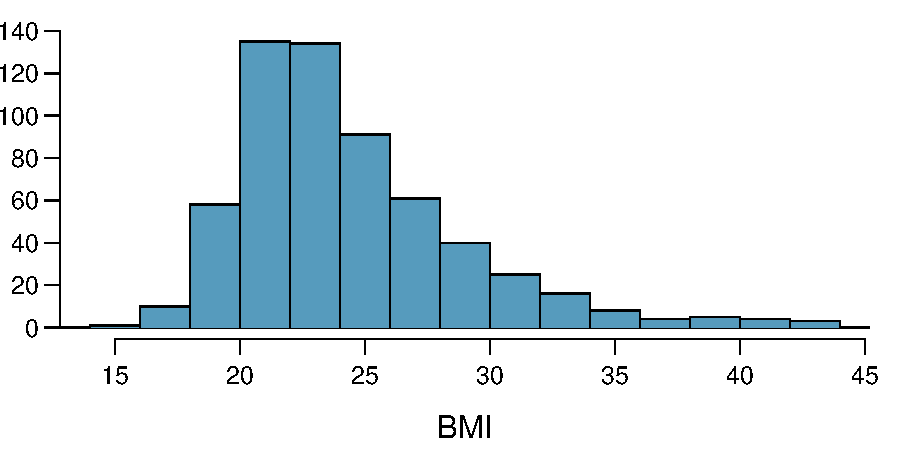
\includegraphics[width=0.7\textwidth]{ch_inference_foundations_oi_biostat/figures/eoce/famussbmi/famussbmi}
\end{center}\vspaceB{-2mm}
\begin{parts}
\item The average BMI in the sample of 595 students is 24.40, and the sample standard deviation is 4.58. Calculate a 99\% confidence interval for the average BMI of college students. What is the interpretation of this confidence interval? What is the margin of error?\\
Determine whether the following statements are true or false, and explain your reasoning. 
\item We are 90\% confident that the average BMI of college students is between 22.09 and 26.71. 
\item We are 90\% confident that the average BMI of 595 students is between 24.09 and 24.71. 
\item The distribution of the BMI observations is right skewed. This invalidates the confidence interval since a confidence interval width is symmetric about the center. 
\item We are 90\% confident that the average BMI of college students is between 24.09 and 24.71. 
\item 90\% of random samples would have a sample mean between 24.09 and 24.71. 
\item The 99\% confidence interval is narrower than the 95\% confidence interval. 
\item In order to decrease the margin of error of a 95\% confidence interval to a fifth of what it is now, the researchers would need to use a sample 5 times larger. 
\item The margin of error at the 90\% level is 0.6. 
\end{parts}
}{}

% 15

\eoce{\qt{Infant Mortality Rates Part I}\label{infantmortal1} Infant mortality rate is the number of deaths of infants under one year old per 1,000 live births. It is often used as an indicator of a country's health level. According to the World Health Organization, the infant morality rate is 32 in 2015. \footnote{\url{http://www.who.int/gho/child_health/mortality/neonatal_infant_text/en/}}
\begin{center}
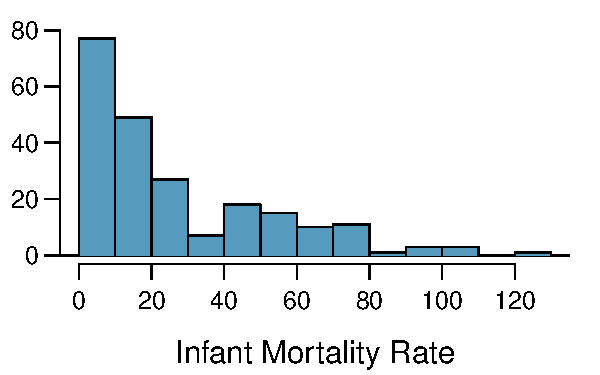
\includegraphics[width=0.7\textwidth]{ch_inference_foundations_oi_biostat/figures/eoce/infantmortal/infantmortal}
\end{center}
The sample mean for 222 countries is 26.70. \footnote{The CIA World Factbook lists 222 countries. We assume that this is a simple random sample and these countries do not comprise of all people in the world (territories etc.). \url{https://www.cia.gov/library/publications/the-world-factbook/rankorder/rawdata_2091.txt}} The sample standard deviation is 25.93. Create a 95\% confidence interval for the average infant morality rate of the world. Verify assumptions. How does this compare to the World Health Organization average?
}{}

% 16
\eoce{\qt{Gifted children, Part II} \label{giftedpt2} Recall the researchers in Exercise~\ref{giftedpt1} investigating characteristics of gifted children and the differences in mother and father IQ. \footfullcite{Graybill:1994}
\begin{parts}
\item Are conditions for inference satisfied in order to construct a confidence interval?
\item Use the point estimate calculated in Exercise~\ref{giftedpt1}. The standard error for the difference in IQ between mother and father is 1.24.\footnote{Paired differences will be covered in Chapter~\ref{inferenceForNumericalData}} Calculate a 95\% confidence interval. 
\item Interpret the confidence interval. Is there anything interesting to comment on?
\end{parts}
}{}

% 17
\eoce{\qt{Working backwards, Part I}\label{backwardspt1} A 90\% confidence interval for a population mean is (65,77). The population distribution is approximately normal and the population standard deviation is unknown. The confidence interval is calculated from a simple random sample of 100 observations. Calculate the sample mean, the margin of error and the sample standard deviation. 
}{}

% 18
\eoce{\qt{Working backwards, Part II}\label{backwardspt2} Consider the 90\% confidence interval for a population mean is (65,77) introduced in Exercise~\ref{backwardspt1}. Calculate the sample mean, the margin of error and the sample standard deviation but from a simple random sample of 35 observations instead. How do the sample mean, marking of error and sample standard deviation compare?
}{}

%19
\eoce{\qt{True or False} Determine if the following statements are true or false, and explain your reasoning. If false, correct the statement so that it is true. 
\begin{parts}
\item If a given value is within a 95\% confidence interval, that value will also be within a 99\% confidence interval. 
\item If a given value is within a 95\% confidence interval, that value will also be within a 90\% confidence interval. 
\item Decreasing the significance level $(\alpha)$ will increase the probability of making a Type 1 error if the confidence interval is testing the null hypothesis under hypothesis testing. 
\item Suppose the null hypothesis is $\mu=5$, and we fail to reject $H_0$. The population parameter is absolutely 5. 
\item Suppose the null hypothesis is $\mu=5$, and the alternative hypothesis is $\mu>5$. We reject the null hypothesis. The population parameter is 2. 
\item Suppose the null hypothesis is $\mu=5$, and the alternative hypothesis is $\mu>5$. We reject the null hypothesis. The population parameter is 7.  
\item An $\alpha$ level of 0.05 is the ideal value for all hypothesis tests. 
\end{parts}
}{}

%20
\eoce{\qt{Heart Transplant Part I}\label{heartpt1} The Stanford University Heart Transplant study was conducted to determine whether an experimental heart transplant program increased lifespan. \footfullcite{Turnbull:1974} Each patient entered the program, and an actual heart transplant occurred between a few weeks to several months after entering the program. \var{survtime} is the number of days patients were alive after the date the patient entered the program until the end date of the study. 
\begin{center}
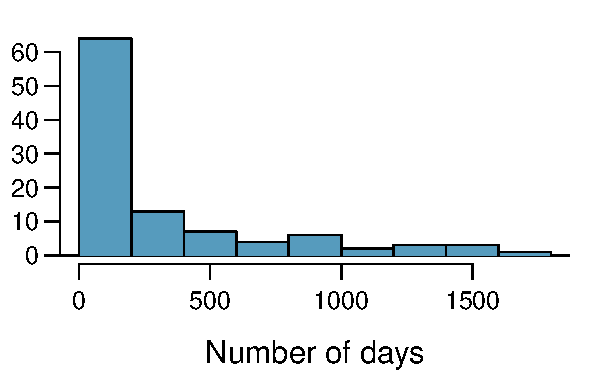
\includegraphics[width=0.7\textwidth]{ch_inference_foundations_oi_biostat/figures/eoce/heartTr/heartTr}
\end{center}
Describe the sample of 103 patients survival time. The sampling distribution of the sample mean of survival time will be 
\begin{parts}
\item right skewed. 
\item left skewed. 
\item a $t$-distribution. 
\item normally distributed. 
\item unknown. 
\end{parts}
}{}

%__________________
\subsection{Hypothesis testing}
% 21
\eoce{\qt{Identifying hypotheses, Part I} Write the null and alternative hypothesis in words and then in mathematical notation for each of the following situations. 
\begin{parts}
\item Recall Exercise~\ref{giftedpt2}. Researchers want to test if there is a difference between the IQ levels of mothers and fathers of gifted children. 
\item Researchers of Exercise~\ref{infantmortal1} want to test if the infant mortality rate is equal to 32, the infant morality rate provided by the WHO in 2015. 
\item The average composite MCAT score in 2004 was 27.1. Is there a noticeable difference between the total MCAT score in 2014 and 10 years ago? \footnote{\url{https://www.aamc.org/download/321494/data/factstable17.pdf}}
\end{parts}
}{}

% 22
\eoce{\qt{Identifying hypotheses, Part II} Write the null and alternative hypothesis in words and then in mathematical notation for each of the following situations. 
\begin{parts}
\item Based on the performance of those who took the GRE exam between July 1, 2004 and June 30, 2007, the average Verbal Reasoning score was calculated to be 462. In 2011 the average verbal score was slightly higher. Do these data provide convincing evidence that the average GRE Verbal Reasoning score has changed since 2004? \footfullcite{webpage:GRE} 
\item The National Sleep Foundation recommends that college students average about 7 hours of sleep per night. Researchers at a community college are interested in showing that students at their school sleep longer than seven hours on average through a sample of students. 
\item Students at Harvard University believe that, on average, students sleep less than 7 hours per night. Do data sampled from the University provided sufficient evidence that they do? 
\end{parts}
}{}

% 23
\eoce{\qt{BRFSS, Part II}\label{brfsspt2} Recall the \data{BRFSS BMI} dataset with sample mean 26.53 and standard deviation 5.84. The CDC in Section~\ref{hypothesisTesting} is curious if the \data{BRFSS BMI} sample provides enough evidence that adults are as healthy as they were 20 years ago. 
\begin{parts}
\item Go through the hypothesis testing framework without the critical value shortcut. What is your conclusion? 
\item How does this result compare to the confidence interval created in Section~\ref{calculate95confidence}?
\end{parts}
}{}

% 24
\eoce{\qt{BRFSS, Part III} Use the sample taken in Exercise~\ref{brfsspt1} instead of \data{BRFSS BMI}. The CDC is now interested in if this new sample provides enough evidence that adults are as healthy as they were 20 years ago. 
\begin{parts}
\item Perform a formal hypothesis test without the critical value shortcut. What is your conclusion? 
\item How does this result compare to the confidence interval created in Section~\ref{calculate95confidence} and the conclusion in Exercise~\ref{brfsspt2}? Why does this make sense?\emph{Hint:} Consider the number of observations in each sample. 
\end{parts}
}{}

% 25
\eoce{\qt{Gifted children, Part III} \label{giftedpt3} The researchers want to test if the sample of IQ levels of the fathers provide evidence that the average IQ of fathers of gift children is larger than the average IQ for the general population, which is 100. A friend outside the study offers to assist in writing the null and alternative hypotheses. Are there any errors? Indicate and correct them. Explain why. \begin{align*}
H_0: \overline{x} = 100\\
H_A: \overline{x} > 100
\end{align*}
}{}

% 26
\eoce{\qt{Infant Morality, Part II} \label{infantmortalpt2} Researchers observed 222 countries' infant mortality rates. They write the following hypotheses to test whether or not the average infant morality rate in the world is 32. 
\begin{align*}
H_0: \overline{x} = 32\\
H_A: \overline{x} < 32
\end{align*}
Is there anything wrong with the hypotheses? If so, explain where they are and correct them.}{}

% 27
\eoce{\qt{Waiting at an ER, Part II} Exercise~\ref{ERwait} provides a 95\% confidence interval for the mean waiting time at an emergency room (ER) of (128 minutes, 147 minutes). 
\begin{parts}
\item A local newspaper claims that the average waiting time at this ER exceeds 3 hours. What do you think of this claim?
\item The Dean of Medicine at this hospital claims the average wait time is 2.2 hours. What do you think of this claim?
\item Without actually calculating the interval, determine if the claim of the Dean from part (b) would be considered reasonable based on a 99\% confidence interval?
\end{parts}
}{}

% 28
\eoce{\qt{Gifted children, Part IV} \label{giftedpt4} The following histogram shows the distribution of the ages (in months) at which these children first counted to 10 successfully from the study introduced in Exercise~\ref{giftedpt2}. Also provided are some sample statistics.\footfullcite{Graybill:1994}

\begin{center}
\begin{minipage}[c]{0.5\textwidth}
\begin{center}
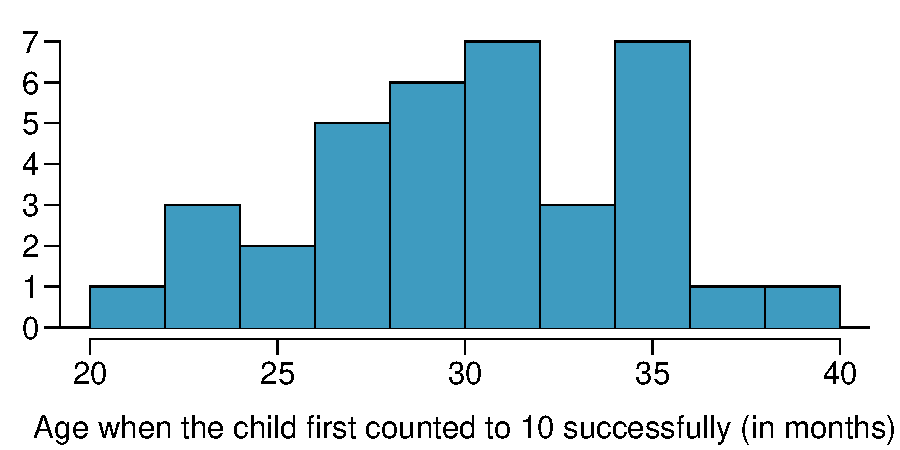
\includegraphics[width=\textwidth]{ch_inference_foundations_oi_biostat/figures/eoce/gifted/gifted_count_hist} 
\end{center}
\end{minipage}
\begin{minipage}[c]{0.1\textwidth}
\begin{tabular}{r | l}
n	& 36 \\
min	& 21 \\
mean	& 30.69 \\
sd	& 4.31 \\
max	& 39 
\end{tabular}
\end{minipage}
\end{center}

\begin{parts}
\item Are conditions for inference satisfied?
\item Suppose you read on a parenting website that children first count to 10 successfully when they are 32 months old, on average. Perform a hypothesis test to evaluate if these data provide convincing evidence that the average age at which gifted children first count to 10 successfully is different than the general average of 32 months. Use a significance level of 0.10.
\item Interpret the p-value in context of the hypothesis test and the data. 
\item Calculate a 90\% confidence interval for the average age at which gifted children first count to 10 successfully.
\item Do your results from the hypothesis test and the confidence interval agree? Explain.
\end{parts}
}{}


% 29
\eoce{\qt{Waiting at an ER, Part III} \label{ERWaitHT} The hospital administrator mentioned in Exercise~\ref{ERwait} randomly selected 64 patients and measured the time (in minutes) between when they checked in to the ER and the time they were first seen by a doctor. The average time is 137.5 minutes and the standard deviation is 39 minutes. He is getting grief from his supervisor on the basis that the wait times in the ER increased greatly from last year's average of 127 minutes. However, the administrator claims that the increase is probably just due to chance. 
\begin{parts}
\item Are conditions for inference met? Note any assumptions you must make to proceed.
\item Using a significance level of $\alpha = 0.05$, is the change in wait times statistically significant? Use a two-sided test since it seems the supervisor had to inspect the data before he suggested an increase occurred.
\item Would the conclusion of the hypothesis test change if the significance level was changed to $\alpha = 0.01$?
\end{parts}
}{}

% 30

\eoce{\qt{Gifted children, Part V}\label{giftedpt5} Exercise~\ref{giftedpt2} describes a study on gifted children. In this study, along with variables on the children, the researchers also collected data on the mother's and father's IQ of the 36 randomly sampled gifted children. The histogram below shows the distribution of mother's IQ.  Also provided are some sample statistics.\\[-2mm]
\begin{minipage}[c]{0.43\textwidth}
\begin{parts}
\item Perform a hypothesis test to evaluate if these data provide convincing evidence that the average IQ of mothers of gifted children is different than the average IQ for the population at large, which is 100. Use a significance level of 0.10.
\item Calculate a 90\% confidence interval for the average IQ of mothers of gifted children.
\item Do your results from the hypothesis test and the confidence interval agree? Explain.
\end{parts}
\end{minipage}
\begin{minipage}[c]{0.56\textwidth}
\begin{center}
{\small\begin{tabular}{r | l}
n	& 36 \\
min	& 101 \\
mean	& 118.2 \\
sd	& 6.5 \\
max	& 131 
\end{tabular}} \\
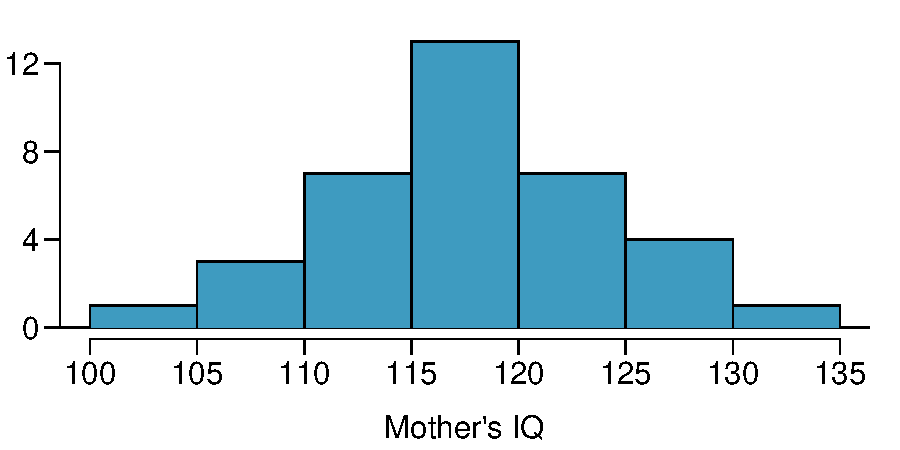
\includegraphics[width=0.94\textwidth]{ch_inference_foundations_oi_biostat/figures/eoce/gifted/gifted_momIQ_hist}
\end{center}
\end{minipage}\vspaceB{-2mm}
}{}

% 31
\eoce{\qt{Nutrition labels} The nutrition label on a bag of potato chips says that a one ounce (28 gram) serving of potato chips has 130 calories and contains ten grams of fat, with three grams of saturated fat. A random sample of 35 bags yielded a sample mean of 134 calories with a standard deviation of 17 calories. Is there evidence that the nutrition label does not provide an accurate measure of calories in the bags of potato chips?  The independence, sample size, and skew conditions have already been verified.
}{}


%32

\eoce{\qt{BRFSS, Part IV} \label{brfsspt4} Using the data observed in Exercise~\ref{brfsspt2}. \begin{parts}
\item The WHO announces that the average adult BMI is 28.5. What do you think of this claim? 
\item Would the WHO's claim be considered reasonable based on a 90\% confidence interval? Why or why not? 
\item What is the lowest confidence interval such that the claim will still be considered reasonable? 
\end{parts}
}{}

% 33

\eoce{\qt{Find the sample mean} You are given the following hypotheses: $H_0$: $\mu = 34$, $H_A$: $\mu > 34$. We know that the sample standard deviation is 10 and the sample size is 65. For what sample mean would the p-value be equal to 0.05? Assume that all conditions necessary for inference are satisfied.
}{}

% 34

\eoce{\qt{Testing for food safety} A food safety inspector is called upon to investigate a restaurant with a few customer reports of poor sanitation practices. The food safety inspector uses a hypothesis testing framework to evaluate whether regulations are not being met. If he decides the restaurant is in gross violation, its license to serve food will be revoked.
\begin{parts}
\item Write the hypotheses in words.
\item What is a Type 1 error in this context?
\item What is a Type 2 error in this context?
\item Which error is more problematic for the restaurant owner? Why?
\item Which error is more problematic for the diners? Why?
\item As a diner, would you prefer that the food safety inspector requires strong evidence or very strong evidence of health concerns before revoking a restaurant's license? Explain your reasoning.
\end{parts}
}{}

% 35
\eoce{\qt{Testing for Fibromyalgia} A patient named Diana was diagnosed with Fibromyalgia, a long-term syndrome of body pain, and was prescribed anti-depressants. Being the skeptic that she is, Diana didn't initially believe that anti-depressants would help her symptoms. However after a couple months of being on the medication she decides that the anti-depressants are working, because she feels like her symptoms are in fact getting better.
\begin{parts}
\item Write the hypotheses in words for Diana's skeptical position when she started taking the anti-depressants.
\item What is a Type 1 error in this context?
\item What is a Type 2 error in this context?
\item How would these errors affect the patient?
\end{parts}
}{}


% 36

\eoce{\qt{Speed reading, Part I} \label{speedReading} Previous literature has shown that online speed reading courses can increase their speed of reading. A company claims that students who take their courses show a 5 times (500\%) increase in the number of words they can read in a minute without losing comprehension. A random sample of 100 students yielded an average increase of 415\% with a standard deviation of 220\%. Is there evidence that the company's claim is false?
\begin{parts}
\item Are conditions for inference satisfied?
\item Perform a hypothesis test evaluating if the company's claim is reasonable or if the true average improvement is less than 500\%. Make sure to interpret your response in context of the hypothesis test and the data. Use $\alpha = 0.025$.
\item Calculate a 95\% confidence interval for the average increase in the number of words students can read in a minute without losing comprehension.
\item Do your results from the hypothesis test and the confidence interval agree? Explain.
\end{parts}
}{}

% 37

\eoce{\qt{Errors in drug testing} Suppose regulators monitored 403 drugs last year, each for a particular adverse response. For each drug they conducted a single hypothesis test with a significance level of 5\% to determine if the adverse effect was higher in those taking the drug than those who did not take the drug; the regulators ultimately rejected the null hypothesis for 42 drugs.
\begin{parts}
\item Describe the error the regulators might have made for a drug where the null hypothesis was rejected.
\item Describe the error regulators might have made for a drug where the null hypothesis was not rejected.
\item Suppose the vast majority of the 403 drugs do not have adverse effects. Then, if you picked one of the 42 suspect drugs at random, about how sure would you be that the drug really has an adverse effect?
\item Can you also say how sure you are that a particular drug from the 361 where the null hypothesis was not rejected does not have the corresponding adverse response?
\end{parts}
}{}


%__________________
\subsection{A Primer on the $t$-distribution (Special Topic)}

%38
\eoce{\qt{Find the p-value, Part I\label{find_T_pval_1}} An independent random 
sample is selected from an approximately normal population with an unknown 
standard deviation. Find the p-value for the given set of hypotheses and $T$ 
test statistic. Also determine if the null hypothesis would be rejected 
at $\alpha = 0.05$.\vspace{-3mm}
\begin{parts}
\item $H_A: \mu > \mu_0 $, $n = 11$, $T = 1.91$
\item $H_A: \mu < \mu_0 $, $n = 17$, $T = -3.45$
\item $H_A: \mu \ne \mu_0 $, $n = 7$, $T = 0.83$
\item $H_A: \mu > \mu_0 $, $n = 28$, $T = 2.13$
\end{parts}
}{}

%39
\eoce{\qt{Working backwards, Part III}\label{backwardspt3} Consider the 90\% confidence interval for a population mean is (65,77) introduced in Exercise~\ref{backwardspt1}. Calculate the sample mean, the margin of error and the sample standard deviation but from a simple random sample of 20 observations instead. How do the sample mean, marking of error and sample standard deviation compare?
}{}


% 40
 
\noindent \begin{minipage}[c]{0.5\textwidth}
\eoce{\qt{$t$-distribution\label{t_distribution}} The figure on the right shows 
three unimodal and symmetric curves: the standard normal (z) distribution,  
the $t$-distribution with 5 degrees of freedom, and the $t$-distribution with 
1 degree of freedom. Determine which is which, and explain your reasoning.}
{}
\end{minipage}
\begin{minipage}[c]{0.48\textwidth}
\begin{center}
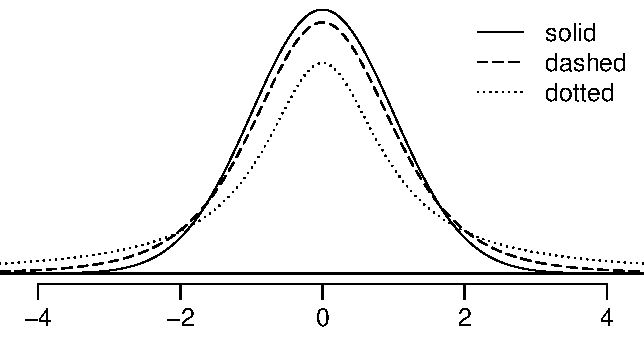
\includegraphics[width=0.93\textwidth]{ch_inference_foundations_oi_biostat/figures/eoce/t_distribution/t_distribution.pdf}
\end{center}
\end{minipage}

% 41
\eoce{\qt{Identify the critical $t$\label{identify_critical_t}} An independent 
random sample is selected from an approximately normal population with unknown 
standard deviation. Find the degrees of freedom and the critical $t$-value 
(t$^\star$) for the given sample size and confidence level.\vspace{-3mm}
\begin{parts}
\item $n = 6$, CL = 90\%
\item $n = 21$, CL = 98\%
\item $n = 29$, CL = 95\%
\item $n = 12$, CL = 99\%
\end{parts}
}{}



% 42

\eoce{\qt{Find the p-value, Part II\label{find_T_pval_2}} An independent 
random sample is selected from an approximately normal population with an 
unknown standard deviation. Find the p-value for the given set of hypotheses 
and $T$ test statistic. Also determine if the null hypothesis would be 
rejected at $\alpha = 0.01$.
\begin{parts}
\item $H_A: \mu > 0.5$, $n = 26$, $T = 2.485$
\item $H_A: \mu < 3$, $n = 18$, $T = 0.5$
\end{parts}
}{}



% 43

\eoce{\qt{Find the mean\label{find_mean}} You are given the following hypotheses:
\begin{align*}
H_0&: \mu = 60 \\
H_A&: \mu \neq 60
\end{align*}
We know that the sample standard deviation is 8 and the sample size is 20. For 
what sample mean would the p-value be equal to 0.05? Assume that all conditions 
necessary for inference are satisfied.
}{}
% 44

\eoce{\qt{$t^\star$ vs. $z^\star$\label{critical_t_vs_z}} For a given confidence 
level, $t^{\star}_{df}$ is larger than $z^{\star}$. Explain how $t^{*}_{df}$ 
being slightly larger than $z^{*}$ affects the width of the confidence interval.
}{}



%__________________
\subsection{Examining the Central Limit Theorem}

% 45

\eoce{\qt{Counties, Part I} \label{countiespt1}  The CDC is concerned largely over minority health and health equity. "Some minorities experience a disproportionate burden of preventable disease, death and disability compared to non-minorities." \footnote{\url{http://www.cdc.gov/minorityhealth/index.html}} Asians are the only racial segment to have cancer as the leading cause of death. Asian American women screen less for breast cancer. The CDC hypothesizes that these results could be explained partially through community and environmental factors. The U.S. Census aggregates data on all 3143 counties in the U.S. including percent of Asians per county. \footnote{SOURCE}
\noindent\begin{minipage}[c]{0.5\textwidth}
\begin{parts}
\item Recreate the distribution of Percent Asian from the \textsf{openintro R} library. The dataset is \textsf{countyComplete}. 
\item Describe the distribution.
\item Sampling distributions for means from simple random samples of 5, 30, and 100 counties is shown in the histograms below. Describe the shapes of these distributions and comment on whether they look like what you would expect to see based on the Central Limit Theorem.
\end{parts}\vspace{3mm}
\end{minipage}
\begin{minipage}[c]{0.5\textwidth}
\begin{center}
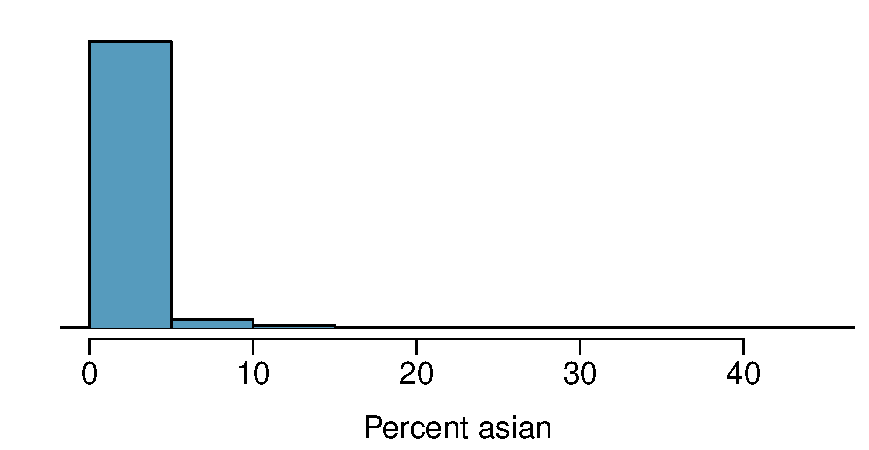
\includegraphics[width=\textwidth]{ch_inference_foundations_oi_biostat/figures/eoce/counties/countyasian} 
\end{center}
\end{minipage}\vspace{-1mm}
\begin{center}
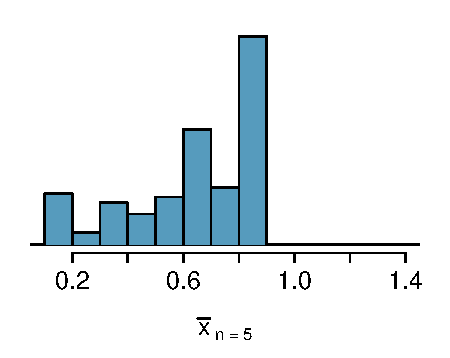
\includegraphics[width=0.325\textwidth]{ch_inference_foundations_oi_biostat/figures/eoce/counties/countyasian_n5} 
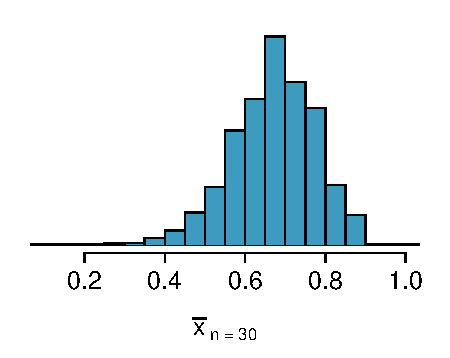
\includegraphics[width= 0.325\textwidth]{ch_inference_foundations_oi_biostat/figures/eoce/counties/countyasian_n30} 
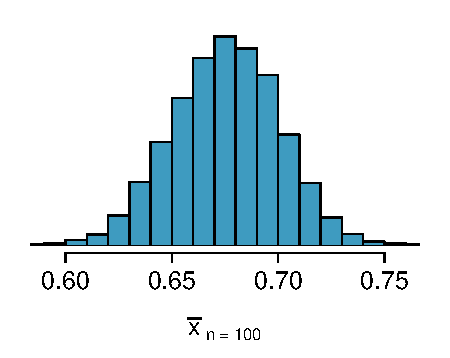
\includegraphics[width= 0.325\textwidth]{ch_inference_foundations_oi_biostat/figures/eoce/counties/countyasian_n100} 
\end{center}
}{}

%46
\eoce{\qt{Counties, Part II} \label{countiespt2}  African Americans experienced high death rates of heart disease and stroke, more than any other racial and ethnic population. They also experience high levels of hypertension, obesity, and diabetes. Infants of African American women have the largest death rate, more than twice that of white women. \footnote{\url{http://www.cdc.gov/minorityhealth/populations/REMP/black.html}} The CDC hopes to gain insight from the population distribution of African Americans in U.S. counties. \\
\noindent\begin{minipage}[c]{0.5\textwidth}
\begin{parts}
\item Find the mean and median of the distribution of Percent Black from the \textsf{openintro R} library. The dataset is \textsf{countyComplete}. Which one is larger? Is this consistent with the distribution skewness?
\item Describe the distribution.
\item Sampling distributions for means from simple random samples of 5, 30, and 100 counties is shown in the histograms below. Describe the shapes of these distributions and comment on whether they look like what you would expect to see based on the Central Limit Theorem.
\end{parts}\vspace{3mm}
\end{minipage}
\begin{minipage}[c]{0.5\textwidth}
\begin{center}
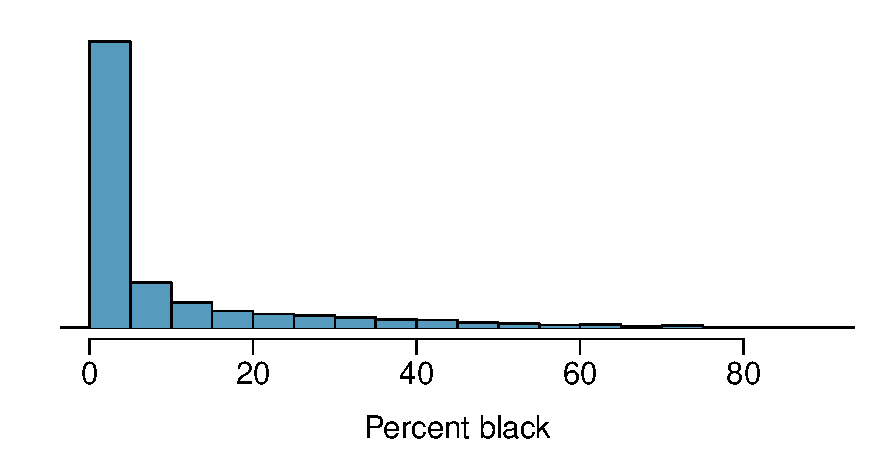
\includegraphics[width=\textwidth]{ch_inference_foundations_oi_biostat/figures/eoce/counties/countyblack} 
\end{center}
\end{minipage}\vspace{-1mm}
\begin{center}
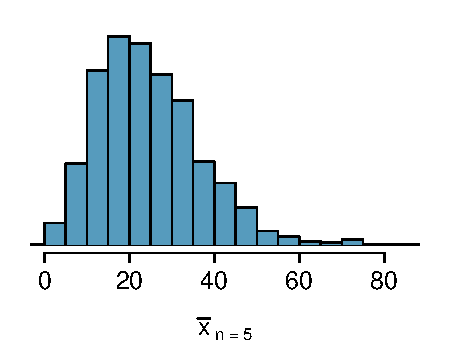
\includegraphics[width=0.325\textwidth]{ch_inference_foundations_oi_biostat/figures/eoce/counties/countyblack_n5} 
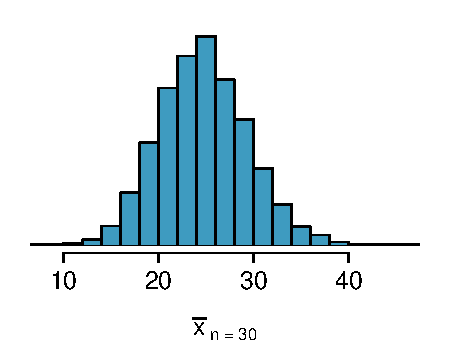
\includegraphics[width= 0.325\textwidth]{ch_inference_foundations_oi_biostat/figures/eoce/counties/countyblack_n30} 
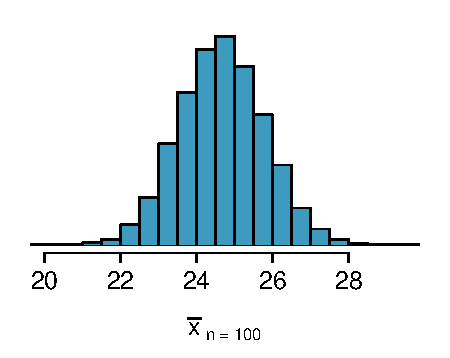
\includegraphics[width= 0.325\textwidth]{ch_inference_foundations_oi_biostat/figures/eoce/counties/countyblack_n100} 
\end{center}
}{}


% 47

\eoce{\qt{Counties, Part III}\label{countiespt3} The maximum value for the percent of Asian in a county from Exercise~\ref{countiespt1} is 43.9\%. The mean is 1.16\%. Calculate the standard deviation of the population in \textsf{R}. Using the Central Limit Theorem, calculate the means and standard deviations of the distribution of the mean from random samples of size 5, 30, and 100. Comment on whether the sampling distributions shown in Exercise~\ref{countiespt1} agree with the values just computed.
}{}

% 48

\eoce{\qt{Counties, Part IV}\label{countiespt4} The maximum value for the percent of African Americans in a county from Exercise~\ref{countiespt2} is 85.7\%. Calculate the standard deviation and standard error.  
Using the Central Limit Theorem, calculate the means and standard deviations of the distribution of the mean from random samples of size 5, 30, and 100. Comment on whether the sampling distributions shown in Exercise~\ref{countiespt2} agree with the values just computed.
}{}
% 49

\eoce{\qt{Identify distributions, Part I} Four plots are presented below. The plot at the top is a distribution for a population. The mean is 10 and the standard deviation is 3. Also shown below is a distribution of (1) a single random sample of 100 values from this population, (2) a distribution of 100 sample means from random samples with size 5, and (3) a distribution of 100 sample means from random samples with size 25. Determine which plot (A, B, or C) is which and explain your reasoning.
\begin{center}
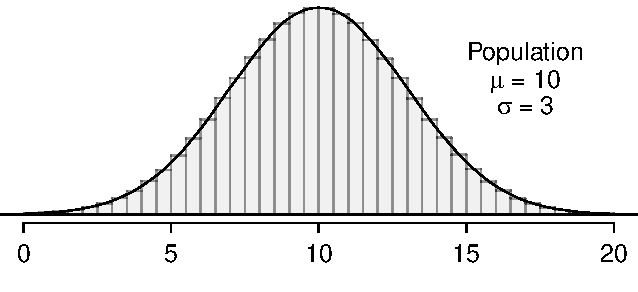
\includegraphics[width=0.5\textwidth]{ch_inference_foundations_oi_biostat/figures/eoce/cltSimSYM/cltSimSYM_pop}
\end{center}
\begin{center}
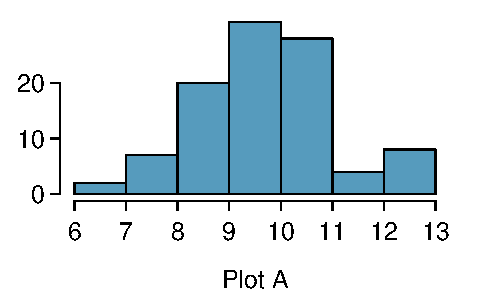
\includegraphics[width=0.32\textwidth]{ch_inference_foundations_oi_biostat/figures/eoce/cltSimSYM/cltSimSYM_n5}
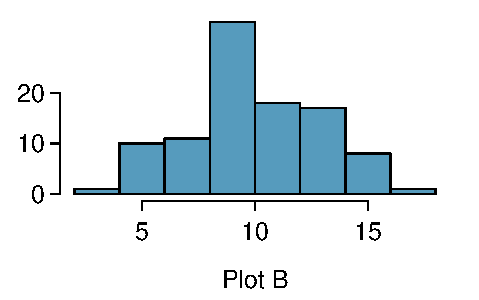
\includegraphics[width=0.32\textwidth]{ch_inference_foundations_oi_biostat/figures/eoce/cltSimSYM/cltSimSYM_samp}
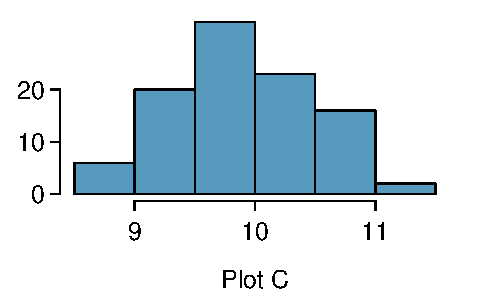
\includegraphics[width=0.32\textwidth]{ch_inference_foundations_oi_biostat/figures/eoce/cltSimSYM/cltSimSYM_n25}
\end{center}
}{}

% 50

\eoce{\qt{Identify distributions, Part II} Four plots are presented below. The plot at the top is a distribution for a population. The mean is 60 and the standard deviation is 18. Also shown below is a distribution of (1) a single random sample of 500 values from this population, (2) a distribution of 500 sample means from random samples of each size 18, and (3) a distribution of 500 sample means from random samples of each size 81. Determine which plot (A, B, or C) is which and explain your reasoning.
\begin{center}
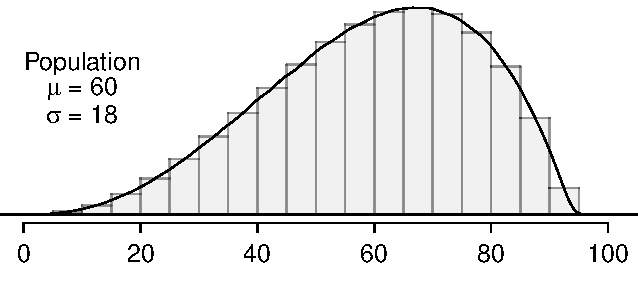
\includegraphics[width=0.5\textwidth]{ch_inference_foundations_oi_biostat/figures/eoce/cltSimLS/cltSimLS_pop}
\end{center}
\begin{center}
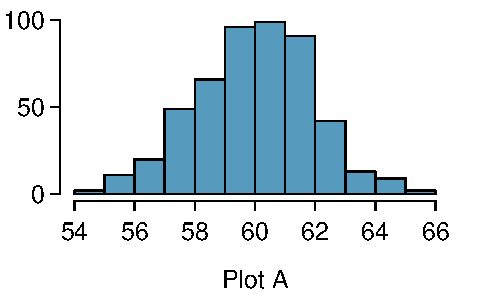
\includegraphics[width=0.32\textwidth]{ch_inference_foundations_oi_biostat/figures/eoce/cltSimLS/cltSimLS_n81}
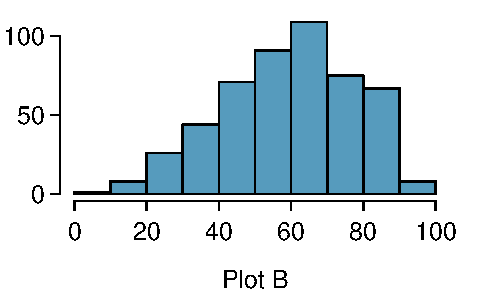
\includegraphics[width=0.32\textwidth]{ch_inference_foundations_oi_biostat/figures/eoce/cltSimLS/cltSimLS_samp}
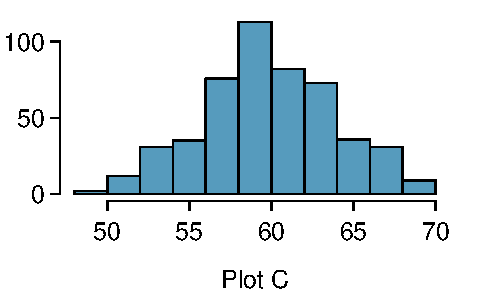
\includegraphics[width=0.32\textwidth]{ch_inference_foundations_oi_biostat/figures/eoce/cltSimLS/cltSimLS_n18}
\end{center}
}{} 

%51

\eoce{\qt{Counties, Part V} \label{countiespt5} The U.S. Census also maps out the distribution of percent White in U.S. counties. The average percent White in a county is 82.89\% with a standard deviation of 16.85\%. The median is 89.1\%
\begin{parts}
\item Is the distribution of percent White in counties symmetric, right skewed, or left skewed?
\item Would you expect most counties in the U.S. to have more or less than 82.89\% White?
\item The U.S. Census is particularly interested in Sheboygan County and its distribution of race. What is the probability that the percent of white people in Sheboygan County is more than 95\% under the normal distribution?
\item What is the probability that the mean percent of whites in 30 randomly chosen counties is more than 99\%?
\item How would doubling the sample size to 60 affect the standard error of the mean?
\item What is the probability that the mean percent of whites in 60 randomly chosen counties is more than 99\%?
\item Does the Central Limit Theorem make sense in this context?
\end{parts}
}{}

% 52

\eoce{\qt{Counties, Part VI} \label{countiespt6} The frequency of children born of two or more races is becoming more and more common. The U.S. Census collected data on the proportion of the population of each county that identifies as more than one race. The average percent per county is 1.98\% and the median 1.6\%. There were no counties with more than 30\% of the population comprised of residents who were two or more race. 
\begin{parts}
\item Is the distribution symmetric, right skewed, or left skewed?
\item Would you expect most counties in the U.S. to have more or less than 1.6\% of the residents two or more races?
\item The U.S. Census is particularly interested in Brookfield County and its distribution of race. What is the probability that the percent of mixed race people in Brookfield County is less than 2\% under the normal distribution?
\item What is the probability that 40 randomly chosen counties have an average that is less than 5\%?
\item How would decreasing the sample size by half affect the standard error of the mean?
\item What is the probability that 20 randomly chosen counties have an average that is less than 5\%?
\item Sketch the two distributions (population and sampling with 40) on the same scale. 
\end{parts}
}{}


\textB{\newpage}

%__________________
\subsection{Inference for other estimators}

% 53

\eoce{\qt{North Carolina births, Part I} \label{ncbirthpt1} North Carolina released birth records in 2004. A random sample of 100 births for babies in North Carolina was taken where 50 of the babies had a mother who was not smoker and another 50 where the mother was a smoker. Use the \textsf{births} dataset in the \textsf{openintro} \textsf{R} library
\begin{parts}
\item What are the hypotheses for evaluating if the average birth weight of a baby is different from mothers who smoke versus mothers who do not smoke. What is the point estimate for the difference between the two population means? Calculate the point estimate using \textsf{R}. 
\item North Carolina released a report stating that the observed difference between the sample means is not statistically significant. Explain what this means in context of the hypothesis test and the data.
\item Would you expect a confidence interval for the difference between the two population means to contain 0? Explain your reasoning.
\end{parts}
}{}

% 54
\eoce{\qt{North Carolina births, Part II} \label{ncbirthpt2} Recall Exercise ~\ref{ncbirthpt1}. Medical literature on smoking's effect on baby birth weights suggests that smoking, on average, results in a decrease in a baby's birth weight 
\begin{parts}
\item What are the hypotheses for evaluating if the average birth weight of a baby is higher from mothers who smoke versus mothers who do not smoke. What is the point estimate for the difference between the two population means?
\item Calculate the point estimate using \textsf{R} and the \textsf{births} dataset in the \textsf{openintro} library. The standard error for the difference is 0.26. Create a 95\% confidence interval. 
\item Perform a formal 95\% hypothesis test. Does the conclusion coincide with what was observed from the 95\% confidence interval?
\end{parts}
}{}

% 55
\eoce{\qt{North Carolina births, Part III} \label{ncbirthpt3} The data from Exercise~\ref{ncbirthpt1} on 100 births also included whether or not the baby was born prematurely. Scientists believe that smoking increases the chance of a baby being born premature. 
\begin{parts}
\item What are the hypotheses for evaluating if there is a difference in the percent of babies who are born prematurely because of the smoking status of a mother. 
\item  North Carolina released a report stating that the observed difference between the sample means is statistically significant. Explain what this means in context of the hypothesis test and the data.
\item Would you expect a confidence interval for the difference between the two population means to contain 0? Explain your reasoning. If not, suggest where the difference between the two population means would lie. 
\end{parts}
}{}

% 56

\eoce{\qt{Nearsightedness} It is believed that nearsightedness affects about 8\% of all children. In a random sample of 194 children, 21 are nearsighted.
\begin{parts}
\item Construct hypotheses appropriate for the following question: do these data provide evidence that the 8\% value is inaccurate?
\item What proportion of children in this sample are nearsighted?
\item Given that the standard error of the sample proportion is 0.0195 and the point estimate follows a nearly normal distribution, calculate the test statistic (the Z statistic).
\item What is the p-value for this hypothesis test?
\item What is the conclusion of the hypothesis test?
\end{parts}
}{}

% 57

\eoce{\qt{Possum, Part II}\label{possumpt1} Male and female possums in Australia and New Guinea were observed and their head, skull, total body and tail length were measured. Published in the \textit{Australian Journal of Zoology}, these researchers were interested in if the total length of the body differed between males and females

\begin{parts}
\item Construct hypotheses appropriate for the previous inference question. 
\item Use the \textsf{possum} dataset in \textsf{openintro} library to calculate a point estimate for differences among the 104 observations. Define the hypothesis in part (a) as differences. 
\item Given the standard error is 0.85 and the point estimate follows a nearly normal distribution, calculate the test statistic. 
\item What is the p-value for this hypothesis test?
\item What is the conclusion of a hypothesis test testing at $\alpha = 0.05$?
\end{parts}
}{}


% 58

\eoce{\qt{Possum, Part II}\label{possumpt2} The researchers in Exercise~\ref{possumpt1} believe that the size of the tail would differ between possums found in Victoria and possums found in New South Wales or Queensland. The standard error is 0.34 and the point estimate follows a nearly normal distribution. 
\begin{parts}
\item What are the hypotheses that the researchers want to test. 
\item What is the point estimate for the difference between the two population means? Use \textsf{R} and the \textsf{possum} dataset in the \textsf{openintro} library. 
\item Calculate a 95\% confidence interval. 
\item The p-value for a 95\% hypothesis test is $1.37\times 10^{-7}$. Explain what this means in the context of the hypothesis test and the data. 
\end{parts}
}{}


\textB{\newpage}


%__________________
\subsection{Sample size and power}

% 59

\eoce{\qtq{Which is higher} In each part below, there is a value of interest and two scenarios (I and II). For each part, report if the value of interest is larger under scenario I, scenario II, or whether the value is equal under the scenarios.
\begin{parts}
\item The standard error of $\bar{x}$ when $s = 120$ and (I) n = 25 or (II) n = 125.
\item The margin of error of a confidence interval when the confidence level is (I) 90\% or (II) 80\%.
\item The p-value for a Z statistic of 2.5 when (I) n = 500 or (II) n = 1000.
\item The probability of making a Type 2 error when the alternative hypothesis is true and the significance level is (I) 0.05 or (II) 0.10.
\end{parts}
}{}

% 60

\eoce{\qt{True or false} Determine if the following statements are true or false, and explain your reasoning. If false, state how it could be corrected.
\begin{parts}
\item If a given value (for example, the null hypothesized value of a parameter) is within a 95\% confidence interval, it will also be within a 99\% confidence interval.
\item Decreasing the significance level ($\alpha$) will increase the probability of making a Type 1 error.
\item Suppose the null hypothesis is $\mu = 5$ and we fail to reject $H_0$. Under this scenario, the true population mean is 5.
\item If the alternative hypothesis is true, then the probability of making a Type 2 error and the power of a test add up to 1.
\item With large sample sizes, even small differences between the null value and the true value of the parameter, a difference often called the effect size\index{effect size}, will be identified as statistically significant.
\item A cutoff of $\alpha$ = 0.05 is the ideal value for all hypothesis tests.
\end{parts}
}{}

% 61

\eoce{\qt{Possum, Part III}\label{possumpt3} The researchers from Exercise~\ref{possumpt1} collected the data on 43 female possums. The sample mean and standard deviation of the skull widths in millimeters are 56.59 and 2.57, respectively.
\begin{parts}
\item They would like to conduct another sample but have a margin of error of no more than 0.5 at a 95\% confidence level. How large of a sample should they collect?
\item Instead they would like to have a margin of error of no more than 0.5 at a 99\% confidence level. How large of a sample should he collect? How does this compare with the answer in part (a)? 
\end{parts}
}{}

% 62

\eoce{\qt{Speed reading, Part II} A random sample of 100 students who took online speed reading courses from the company described in Exercise~\ref{speedReading} yielded an average increase in reading speed of 415\% and a standard deviation of 220\%. Researchers would like to calculate a 95\% confidence interval for the average increase in reading speed with a margin of error of no more than 15\%. How many students should they sample?
}{}

% 63

\eoce{\qt{Waiting at the ER, Part IV} Exercise~\ref{ERWaitHT} introduced  a hospital where ER wait times were being analyzed. The previous year's average was 128 minutes. Suppose that this year's average wait time is 135 minutes.
\begin{parts}
\item Provide the hypotheses for this situation in plain language.
\item Assume that the director of the ER wants to collect a sample size of $n=64$, what values could $\bar{x}$ take so that the $H_0$ is rejected? Suppose the sample standard deviation from the earlier exercise (39 minutes) is the population standard deviation. The conditions for the nearly normal model for $\bar{x}$ are already verified. 
\item Calculate the probability of a Type 2 error.
\end{parts}
}{}
